\section{Null model construction}\label{sec:nullmodel}
The kind of data considered in this work comes from RNA Sequencing experiments. This experiments use wet biology methods to extract information from samples. If one imagines it exists an unknown function that describes the gene expression across the samples considered, what experimenters people do is to sample  this function, picking up some genes.

In this section it is described a null model of sampling, this is useful to verify if the data distributions seen are just an effect of this experimental sample or if they carry some useful and interesting information.

As described in~\cite{Mazzolini2018} a random matrix has to be created. This matrix is a collection of components and realizations exactly as~\ref{fig:componetstable}. The values of abundances of each component in each realization $n_{i j}$ are randomly assigned with a probability determined by 
the global abundance in the whole dataset~\ref{eq:abundance}. Values of each column are extracted until the size~\ref{eq:size} is 
reached. Strictly speaking it is a multinomial process
\begin{equation}
P\left({n_i};M\right)=\frac{M!}{\prod_{i=1}^{N} n_i}\prod_{i=1}^N f_i^{n_i}
\end{equation}
where $n_i$ is the number of components with frequency $f_i$, being $f_i=\frac{a_i}{\sum_{i=1}^{N}a_{i}}$ as defined in~\ref{eq:fi}.

Figure~\ref{fig:structure/randomsampling} shows an example of this, $M$ components are picked up with respect to their frequency in the dataset. The most abundant components, which are also the ones with higher frequency (frequency is nothing but the normalised abundance), have a greater probability to be picked up.
\begin{figure}[htb!]
    \centering
    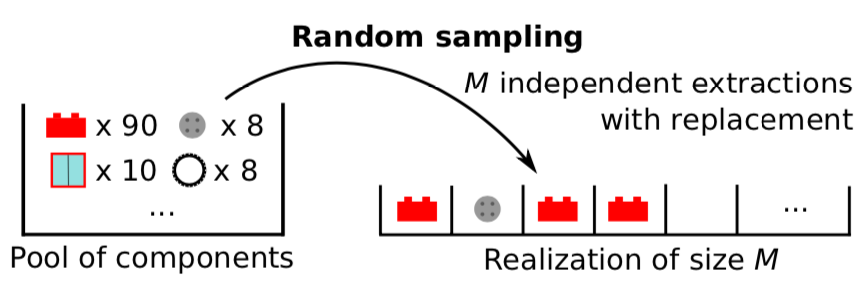
\includegraphics[width=0.8\linewidth]{pictures/structure/randomsampling.png}
    \caption{Random sampling of components to build a realization of size $M$}
    \label{fig:structure/randomsampling}
\end{figure}

Using this construction on data of counts on both dataset, by definition the Zipf's law sampled are identical to the data's one.
\begin{figure}[htb!]
\begin{minipage}{0.5\textwidth}
    \centering
    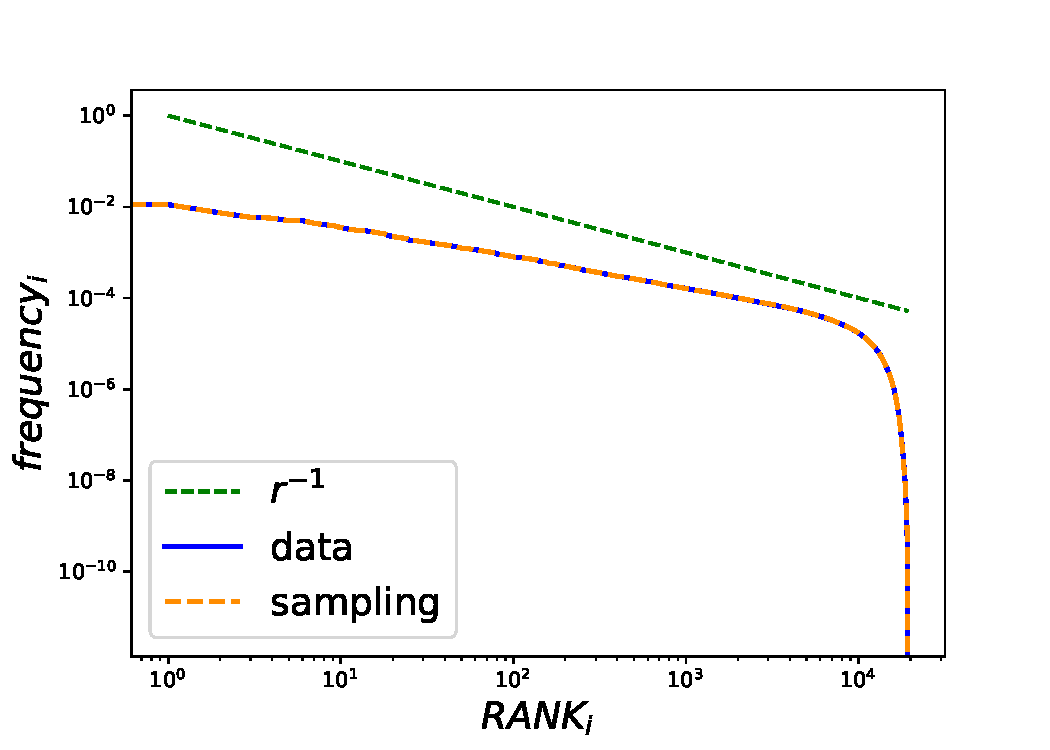
\includegraphics[width=0.95\linewidth]{pictures/structure/tcga/globalzipf_null.pdf}
\end{minipage}
\hspace{2mm}
\begin{minipage}{0.5\textwidth}
    \centering
    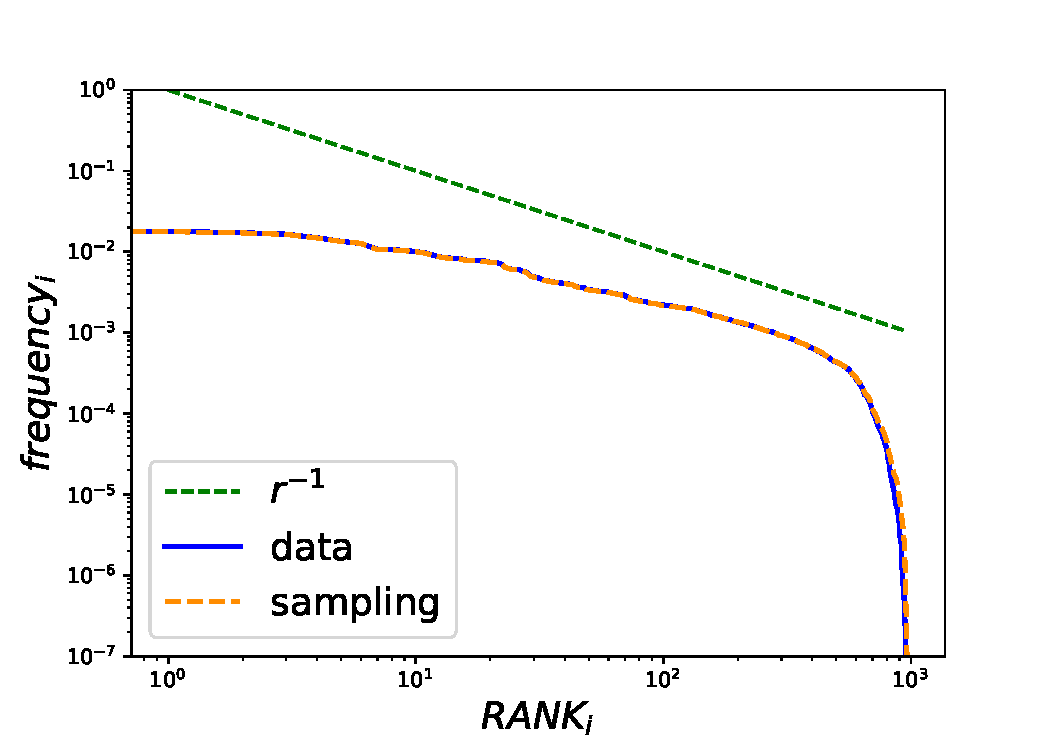
\includegraphics[width=0.95\linewidth]{pictures/structure/gtex/globalzipf_null.pdf}
\end{minipage}
\caption{Zipf's law sampled; TCGA(left) and GTEx (right)}
\label{fig:structure/globalzipf_null}
\end{figure}
By construction the distribution of the sizes of the sampling and of the data are identical.
\begin{figure}[htb!]
\begin{minipage}{0.5\textwidth}
    \centering
    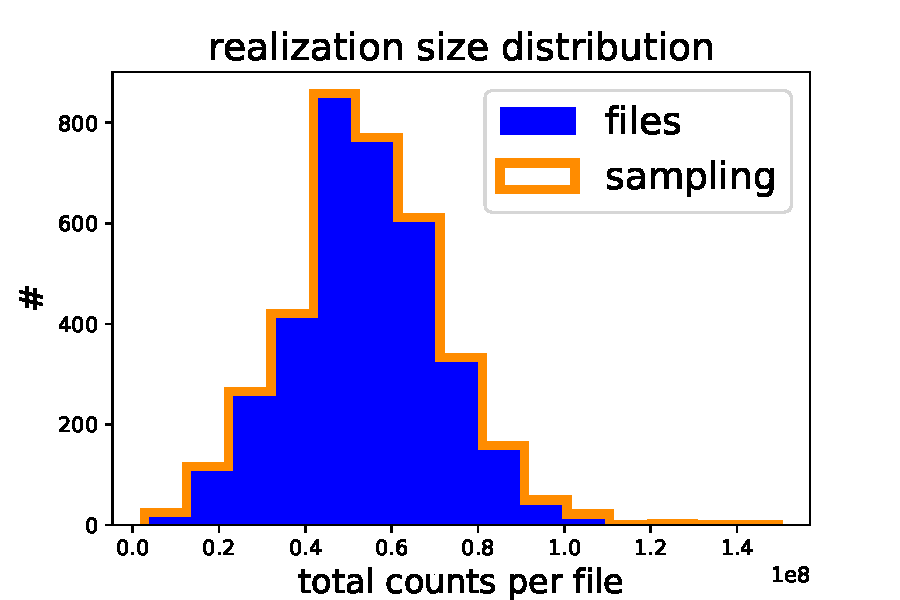
\includegraphics[width=0.95\linewidth]{pictures/structure/tcga/sizeDistr_null.pdf}
\end{minipage}
\hspace{2mm}
\begin{minipage}{0.5\textwidth}
    \centering
    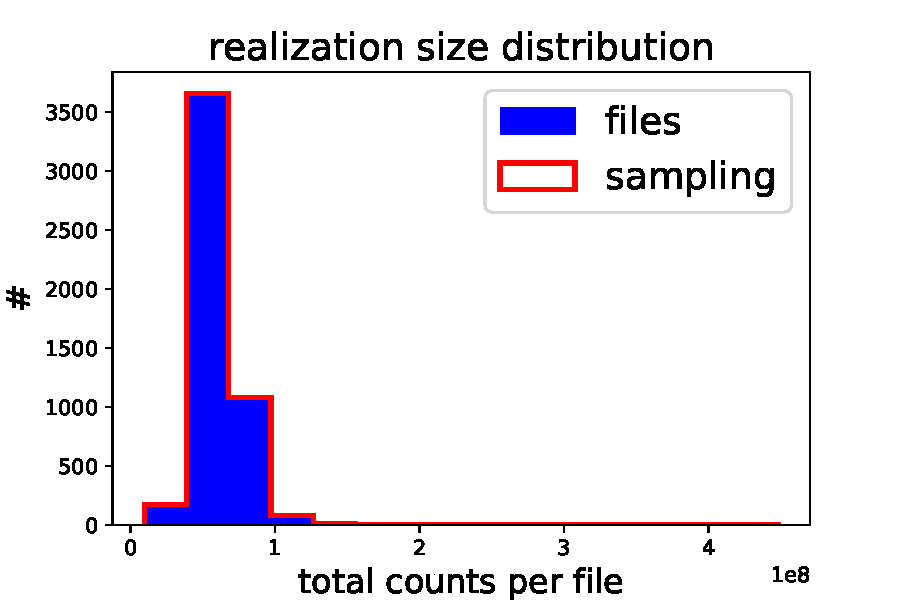
\includegraphics[width=0.95\linewidth]{pictures/structure/gtex/sizeDistr_null.pdf}
    \end{minipage}
\caption{Distribution of sizes $M$; TCGA(left) and GTEx (right)}
    \label{fig:structure/sizeDistr_null}
\end{figure}

Looking at the $U$s, it is evident that data is different from sampling. This is a signal that the null model is not enough to explain the data matrices. In particular from figure~\ref{fig:structure/globalU_null} it is evident that the null model generate the matrices in a manner such that more components have high occurrence with respect to the original data. This can be easily explained, in fact in real world there are some genes that are highly expressed but only in a subset of the whole dataset; these genes are specific for certain type of samples. The null model gets the information the such genes are highly expressed from the abundance and so samples these quite often (components with high abundance have a greater chance to be picked up by the null model sampling).
\begin{figure}[htb!]
\begin{minipage}{0.5\textwidth}
    \centering
    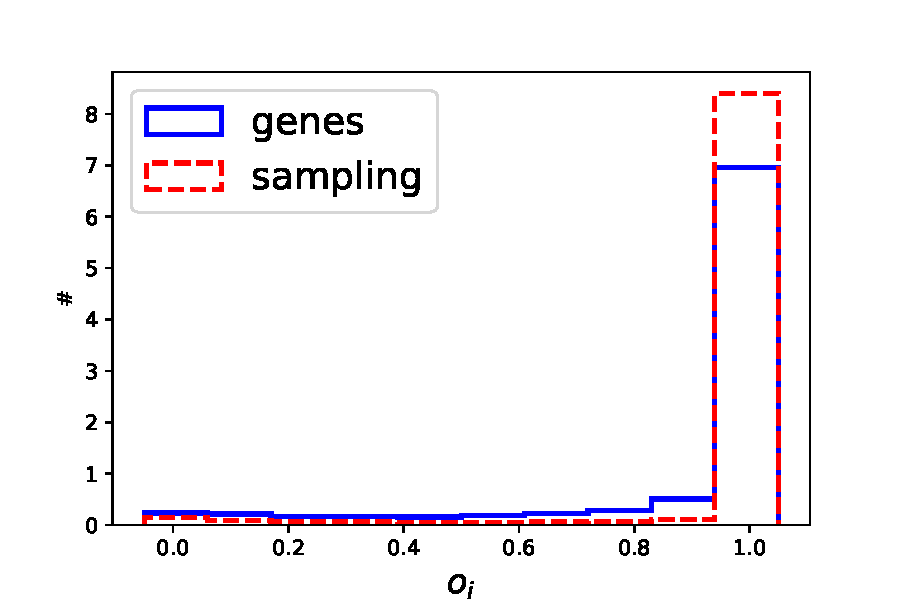
\includegraphics[width=0.95\linewidth]{pictures/structure/tcga/globalU_null.pdf}
\end{minipage}
\hspace{2mm}
\begin{minipage}{0.5\textwidth}
    \centering
    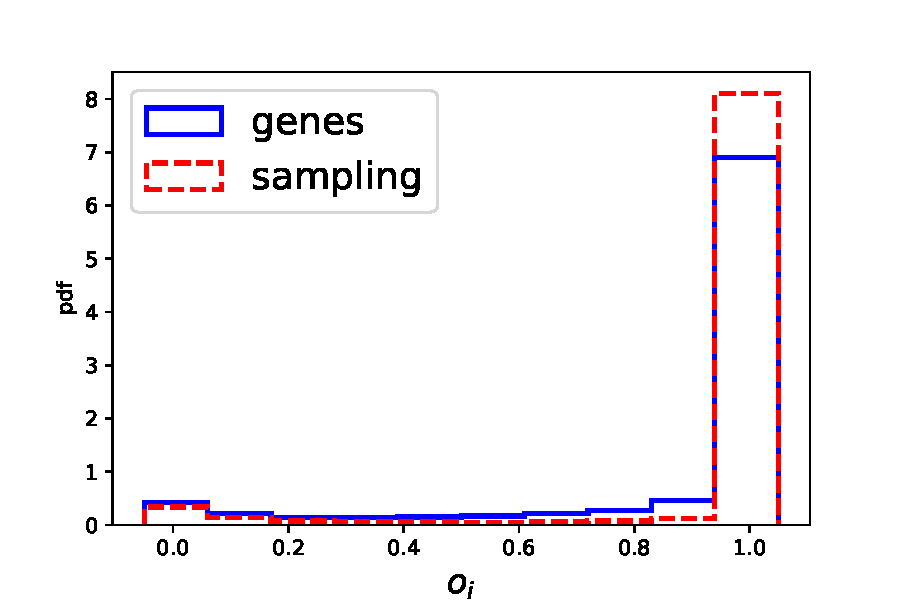
\includegraphics[width=0.95\linewidth]{pictures/structure/gtex/globalU_null.pdf}
    \end{minipage}
\caption{Occurrence distributions; TCGA(left) and GTEx (right)}
\label{fig:structure/globalU_null}
\end{figure}

Looking at the Heaps's law~\cite{Heaps:1978:IRC:539986} 
, again the curves differ and the null model is not enough complete to explain the trend. In figure~\ref{fig:structure/heaps_null} the Heaps's law is presented compared to the one obtained by sampling, note that each data point share the abscissa with a sampling one (figures~\ref{fig:structure/sizeDistr_null} are nothing but the histograms of the abscissas of~\ref{fig:structure/heaps_null}). It happens that the sampling curve is above the data's one. This means that to build a sample of size $M$ just by sampling it is necessary to use a greater number of different genes than the number of different genes actually expressed in nature. In other words in real world are expressed only the genes that are really useful in the sample, and this is not describable just by sampling. This fact is coherent with the fact that the $U$s differ.
\begin{figure}[htb!]
\begin{minipage}{0.5\textwidth}
    \centering
    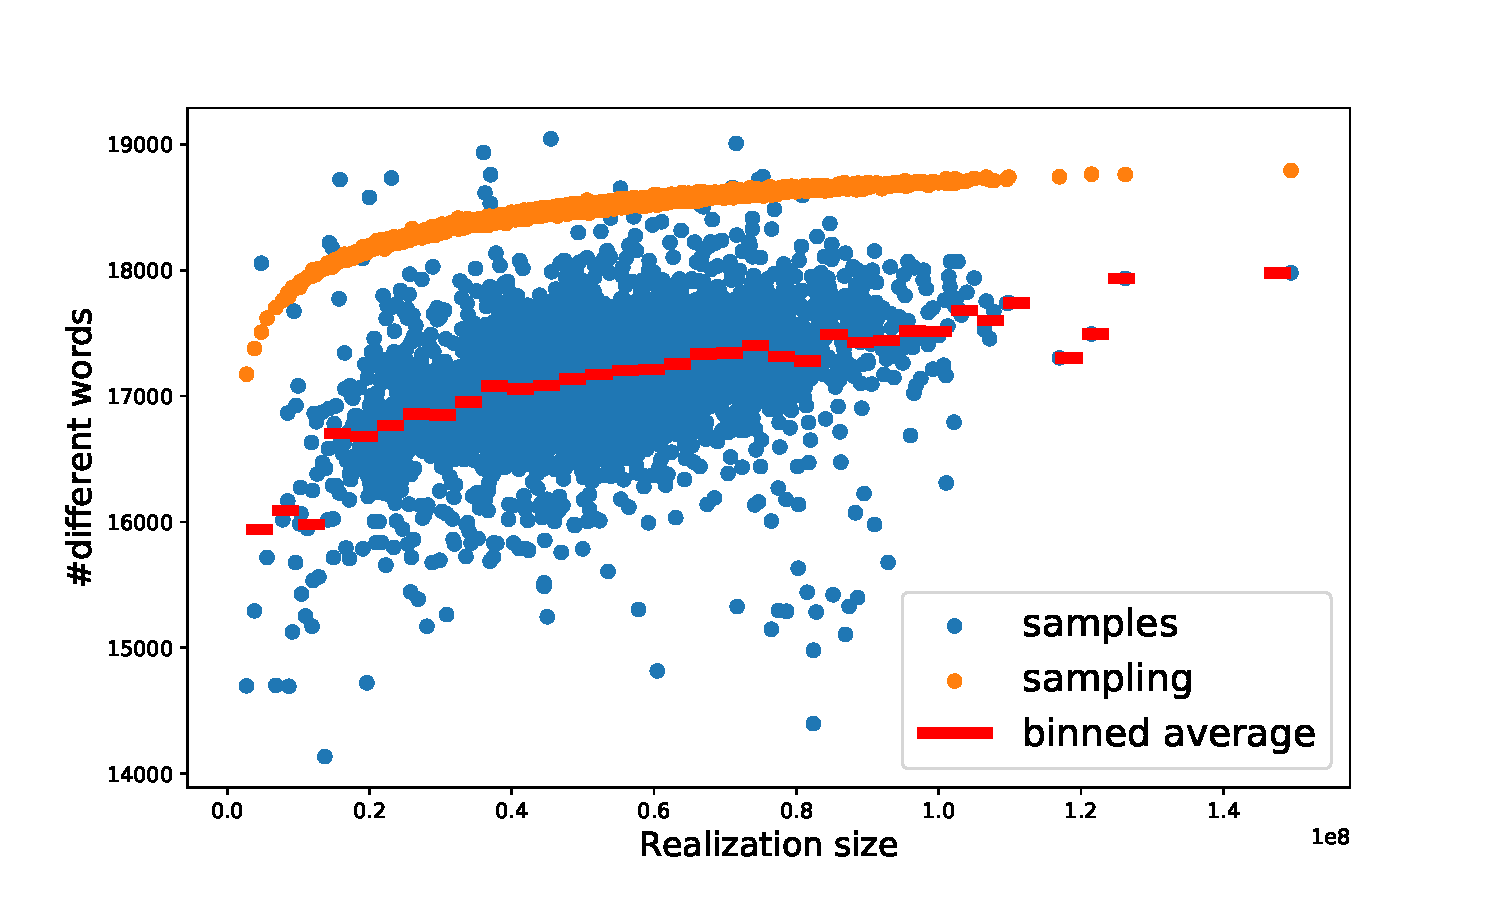
\includegraphics[width=0.95\linewidth]{pictures/structure/tcga/heaps_null.pdf}
    \end{minipage}
\hspace{2mm}
\begin{minipage}{0.5\textwidth}
    \centering
    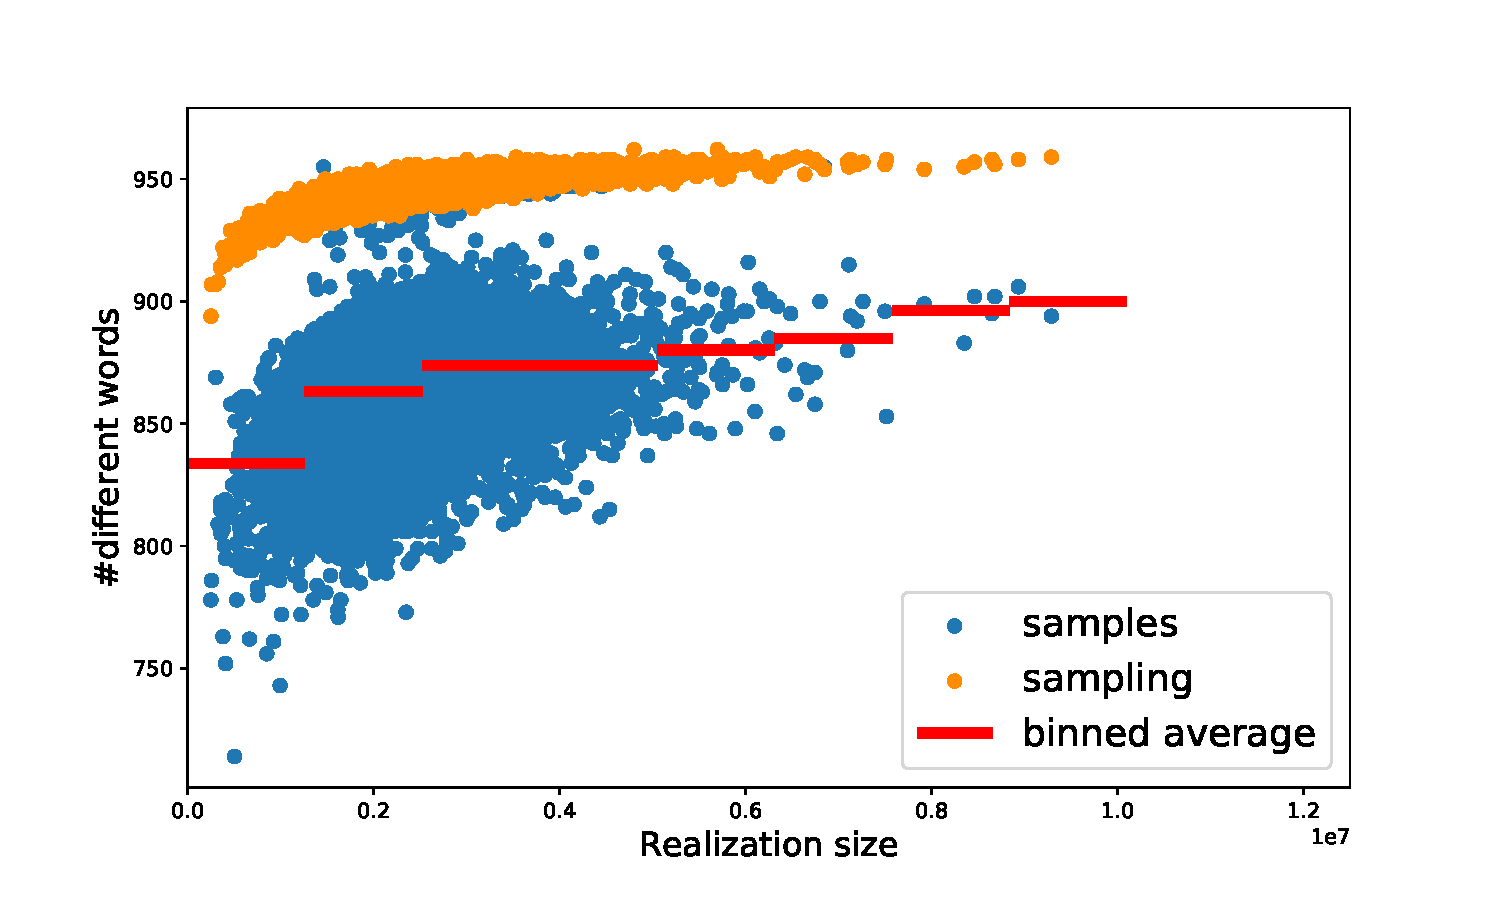
\includegraphics[width=0.95\linewidth]{pictures/structure/gtex/heaps_null.pdf}
    \end{minipage}
\caption{Heaps' law; TCGA(left) and GTEx (right)}
\label{fig:structure/heaps_null}
\end{figure}
Another way to see this is looking at the histograms of the number of different genes expressed, actually the distribution of the~\ref{fig:structure/heaps_null} y axis. Figure~\ref{fig:structure/diffwordsDistr_null} shows that these distributions are completely different if one looks at the data and at the samples.
\begin{figure}[htb!]
\begin{minipage}{0.5\textwidth}
    \centering
    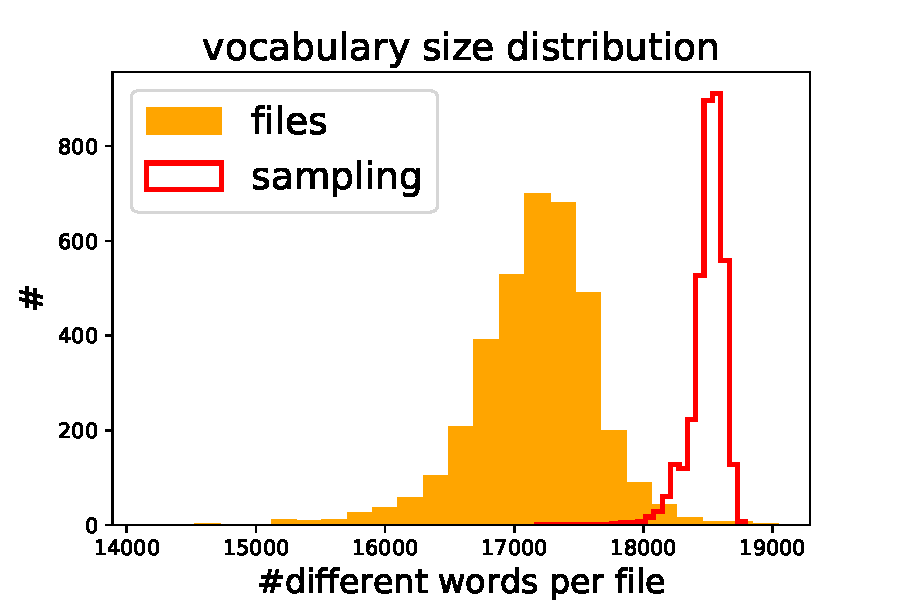
\includegraphics[width=0.95\linewidth]{pictures/structure/tcga/diffwordsDistr_null.pdf}
    \end{minipage}
\hspace{2mm}
\begin{minipage}{0.5\textwidth}
    \centering
    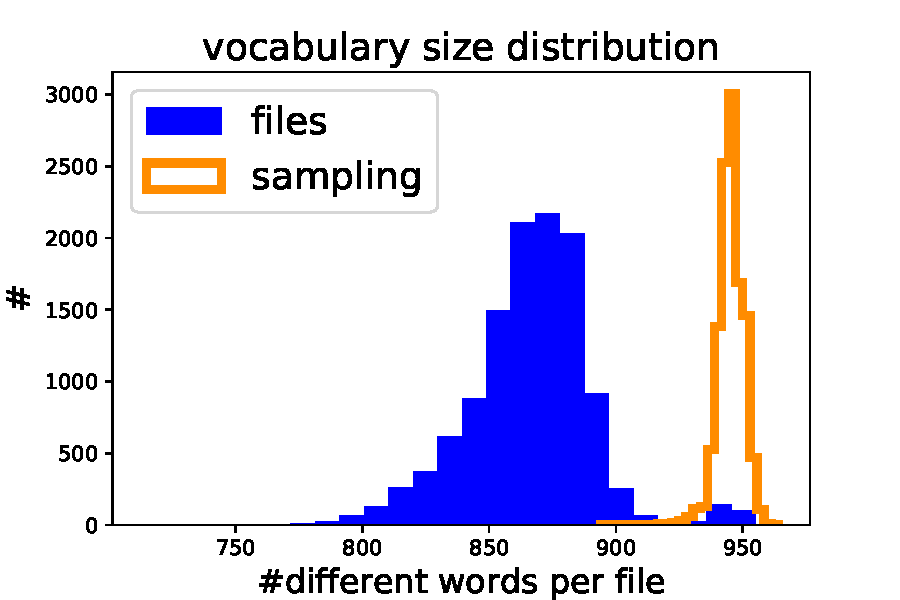
\includegraphics[width=0.95\linewidth]{pictures/structure/gtex/diffwordsDistr_null.pdf}
    \end{minipage}
\caption{Occurrence distributions; TCGA(left) and GTEx (right)}
\label{fig:structure/diffwordsDistr_null}
\end{figure}